\begin{frame}\frametitle{Results}
\begin{Large}
Results
\end{Large}
\begin{itemize}
\item Rating our work
\begin{itemize}
\item Word similarity 
\item Convergence time
\end{itemize}
\item Results
\begin{itemize}
\item Advanced Optimizers
\item Input Shuffling
\end{itemize}
\item Discussion
\begin{itemize}
\item Comparison to Gensim and other related work
\end{itemize}
\end{itemize}
\end{frame}

\begin{frame}
\frametitle{Word similarity}
\begin{Large}
What is word similarity? 
\end{Large}
\medskip
\begin{itemize}
\item Two word embeddings are close to each to other if their cosine distance is small. 
\item Pairs of word rated between 1 and 10 on their similarity, 
\item 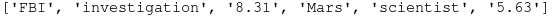
\includegraphics[scale=0.5]{images/wordsim353_example}
\item We are going to rank our model on the corelation between the distance of the word pairs and the human score.
\end{itemize}
\centerline{ 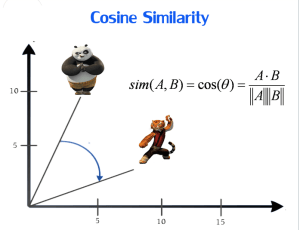
\includegraphics[scale=0.4]{images/cosine}}
\end{frame}
\begin{frame}
\frametitle{Convergence time}
\begin{itemize}
\item Defined convergence time based on word similarity
\item Early Stoppage if: $ \rho -  \rho_{prev} < 0.009$ 
\item No more than 20 epochs. 
\end{itemize}
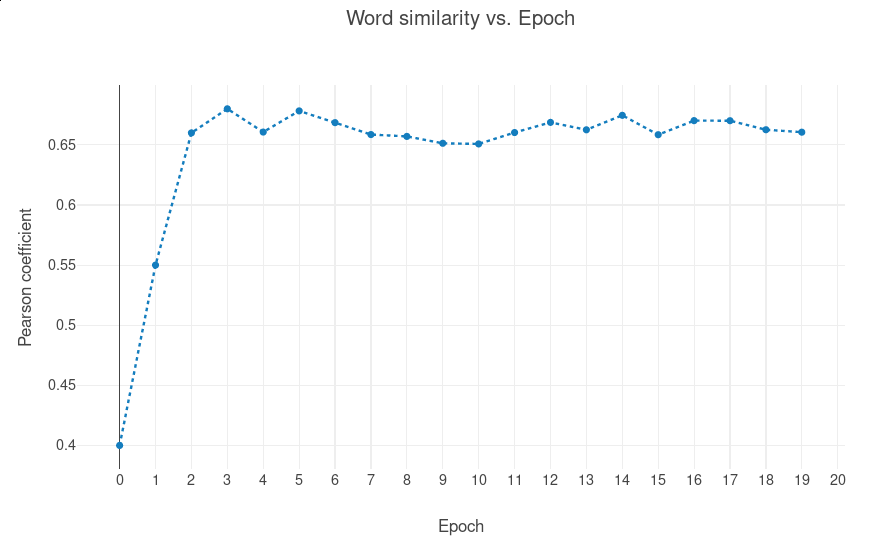
\includegraphics[scale=0.3]{images/wordsim_convergence}
\end{frame}
\begin{frame}
\frametitle{Advanced Optimizers}
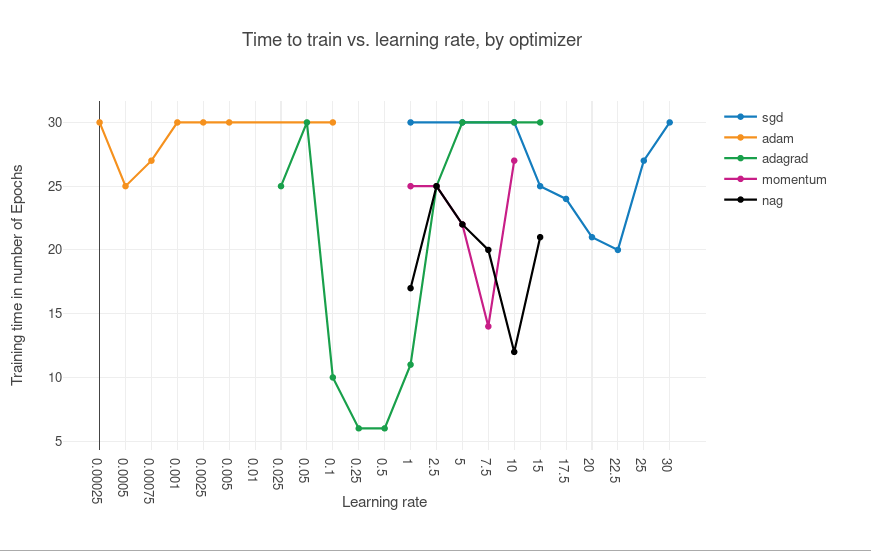
\includegraphics[scale=0.4]{images/results_optim}
\end{frame}
\begin{frame}
\frametitle{Input Shuffling}
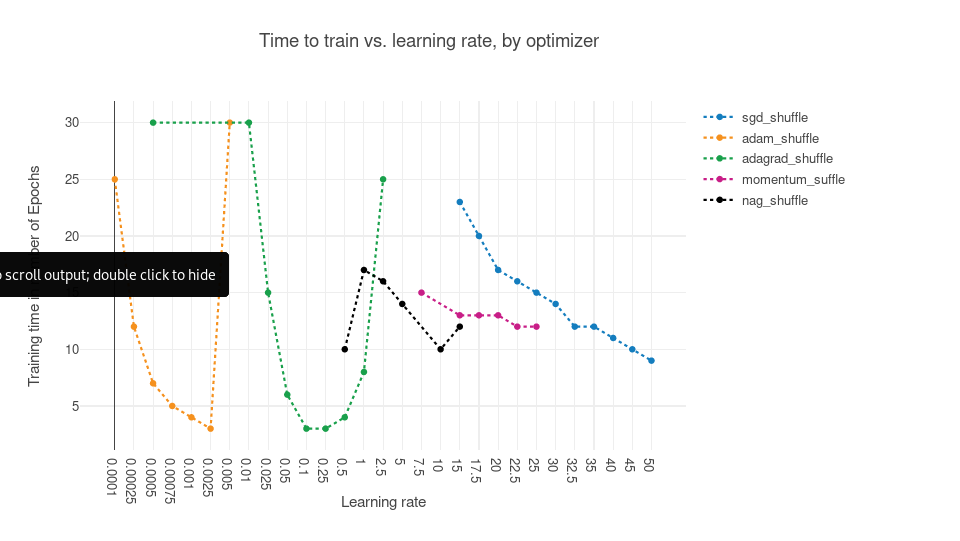
\includegraphics[scale=0.4]{images/results_shuffle}
\end{frame}